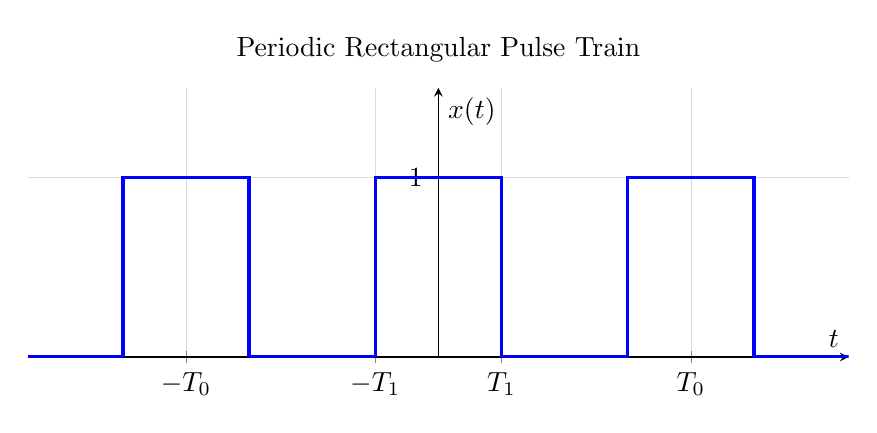
\begin{tikzpicture}
	\begin{axis}[
		width=12cm,
		height=5cm,
		title={Periodic Rectangular Pulse Train},
		xlabel={$t$},
		ylabel={$x(t)$},
		axis lines=middle,
		xmin=-6.5, xmax=6.5,
		ymin=0, ymax=1.5,
		xtick={-4, -1, 1, 4},
		xticklabels={$-T_0$, $-T_1$, $T_1$, $T_0$},
		ytick={1},
		grid=major,
		grid style={line width=.1pt, draw=gray!30},
		]
		
		% Draw the pulses (using representative values T0=4, T1=1)
		% Central Pulse
		\draw[blue, very thick] (axis cs:-1,0) -- (axis cs:-1,1) -- (axis cs:1,1) -- (axis cs:1,0);
		% Next Pulse
		\draw[blue, very thick] (axis cs:3,0) -- (axis cs:3,1) -- (axis cs:5,1) -- (axis cs:5,0);
		% Previous Pulse
		\draw[blue, very thick] (axis cs:-5,0) -- (axis cs:-5,1) -- (axis cs:-3,1) -- (axis cs:-3,0);
		% Zero lines connecting them
		\draw[blue, very thick] (axis cs:-6.5,0) -- (axis cs:-5,0);
		\draw[blue, very thick] (axis cs:-3,0) -- (axis cs:-1,0);
		\draw[blue, very thick] (axis cs:1,0) -- (axis cs:3,0);
		\draw[blue, very thick] (axis cs:5,0) -- (axis cs:6.5,0);
		
		% Add period marker
		\draw[<->, thick] (axis cs:0, -0.3) -- (axis cs:4, -0.3) node[midway, below=2pt] {Period $T_0$};
		
	\end{axis}
\end{tikzpicture}